\documentclass[11pt]{article}

\usepackage{ifpdf}
\ifpdf
    \usepackage[pdftex]{graphicx}   % to include graphics
    \pdfcompresslevel=9
    \usepackage[pdftex,     % sets up hyperref to use pdftex driver
            plainpages=false,   % allows page i and 1 to exist in the same document
            breaklinks=true,    % link texts can be broken at the end of line
            colorlinks=true,
            pdftitle=My Document
            pdfauthor=My Good Self
           ]{hyperref}
    \usepackage{thumbpdf}
\else
    \usepackage{graphicx}       % to include graphics
    \usepackage{hyperref}       % to simplify the use of \href
\fi
\usepackage{mathtools}
\usepackage{float}

\title{COMP5005 Final Project}
\author{Yuanbo Guo 7389051}
\date{\today}

\begin{document}
\maketitle
\newpage
\tableofcontents
\newpage

\begin{abstract}
In this report, the existence of optimal solution has been shown mathematically. Based on that, several schemes are given to approach optimal solution.
\end{abstract}
\section{Problem Statement}
In this task, we aim to build a learning scheme for elevator to minimize the overall waiting time which is:
$$T=T_1+\frac{T_2}{2}$$
where $T_1$ is the time elevator going through waiting floor to a requested floor, $T_2$ is elevator going from get off floor to a desired waiting floor.
The fact $T_1$ has more weight than $T_2$, makes $T_1$ a primary factor in optimization. The expected behaviour of the automaton is the elevator always try go to a close floor near next get on point.

\section{Modelling}
\emph{Note that in this whole article, we use ``$o$'' as a lowercase ``$O$'', not ``zero''}\\

We can view this problem as a stochastic process. An event in this case is a tuple: $$e=(I,O)$$

where random variable $I$ (in) is the floor a person get on and $O$ (out) is the floor get off.\\

Usually, as a common sense, $I$ and $O$ are not independent, which is $P_e(I=i,O=o) \neq P_e(I=i)P_e(O=o)$. In this project we do not have the information $P_e(O|I)$ (however we do not need this information).\\

\subsection{Assumptions}
According to the description of this project, we have the following hypotheses:

\begin{enumerate}
  \item Time is discretized, namely time instance $n$.
  \item The distribution $P(I)$ and $P(O)$ do not change with time.
  \item An elevator can only load one person at a time.
  \item An elevator can only know the next request right after it arrives the desired floor.
  \item Each person is independent to each other so that $e_n$ and $e_{n+1}$ are independent.
  \item The action of elevator choosing which floor to wait for next person does not affect the next person's choice
\end{enumerate}

According to assumption 5 we conclude that this is a memoryless process since each event $e_n$ is independent with respect to time $n$. From this we have:
$$\forall n, P(I(n+1)|O(n))=P(I)P(O)$$

Since we try to optimize waiting time $T$ which is the ``gap'' between two adjacent event $e(n)$ and $e(n+1)$, the above property gives us the most important information we ever wanted! (i.e. we can then solve each floor respectively)

\subsection{Analysis}
Assuming there are $k$ floors. Let $\tilde{X}=[X_1,X_2,...,X_k]$ be the solution vector, where random variable $X_i$ is the floor number elevator choose to go to when its currently position is floor $i$.\\

If a person get off at floor $O$ and the next person is waiting at floor $I$:

\begin{align*}
E(T)&=E[T(O,I,\tilde{X})]\\
&=E[\sum_oT(o,I,X_o)P_O(O=o)]\\
&=E[\sum_o E[\sum_\alpha T(o,I,\alpha) P(X_o=\alpha)]P_O(O=o)]\\
&=\sum_o \sum_\alpha (\sum_iT(o,i,\alpha)P(I=i))P(X_o=\alpha)P_O(O=o)
\end{align*}

where
$$T(o,i,\alpha)=|i-\alpha|+\frac{1}{2}|o-\alpha|$$

Let $\tilde{M}=[M_1,M_2,...,M_k]$ be the $Loss$ vector, where
$$M_o=\sum_\alpha (\sum_iT(o,i,\alpha)P(I=i))P(X_o=\alpha)$$

is the $Loss$ of each floor. we are trying to minimize:
$$E[T(O,I,\tilde{X})]=\sum_oM_oP(O=o)$$

Since each $X \in \tilde{X}$ is unrelated to each other, the above equation is equal to:
$$\text{minimize } M_o, o\in O$$

Let $$\mu_{o,\alpha} = \sum_iT(o,i,\alpha)P(I=i)$$

then we have a simplified expression:
$$\text{minimize }M_o=\sum_\alpha \mu_{o,\alpha} P(X_o=\alpha) \text{ for reach } o\in O$$

Let $\mu_{o,\alpha^*}=min(\mu_{o,\alpha}),P(X_o=\alpha^*)=1$. The minimum $E(T)$ is:
$$E[T]_{min}=E[min(M_o)]=\sum_o\mu_{o,\alpha^*}P(O=o)$$

\emph{Our final goal is to find $\alpha^* \in \alpha$ for each $o \in O$.}

\subsection{Schemes}
Let the ``penalty'' probability be:
$$c_{o,\alpha}=\frac{\mu_{o,\alpha}}{\sum_\alpha\mu_{o,\alpha}}$$

The optimization task becomes:
$$\text{minimize } M_o=\sum_\alpha c_{o,\alpha} P(X_o=\alpha),c_{o,\alpha} \in [0,1], o \in O$$

Now let us look at the general $Loss$ equation in analyzing Learning Automata:
$$E[M(n)]=\sum_i^R c_i p_i(n),c_i \in [0,1]$$

Note that the similarity between this two equations, they are basically the same except that $c_{o,\alpha}$ involves the distribution $P(I)$ to calculate. So we need a little ``hacking(math)'' to fix this:

Let:

$$\hat{\mu}_{o,\alpha}=\sum_iT(o,i,\alpha)$$

Then:

$$\hat{c}_{o,\alpha}=\frac{\mu_{o,\alpha}}{\sum_\alpha\hat{\mu}_{o,\alpha}}$$
$$\hat{M}_o=\sum_\alpha \hat{c}_{o,\alpha} P(X_o=\alpha)$$

Therefore
$$\hat{M}_o=\eta M_o$$

Where
$$\eta=\frac{\sum_\alpha\mu_{o,\alpha}}{\sum_\alpha\hat{\mu}_{o,\alpha}}$$


Since the assumption $P(I)$ is not changing with time, we can easily prove that \emph{$\eta$ is a constant}. \emph{To minimize $M_o$ is equal to minimize $\hat{M}_o$!}\\

Now the problem solved, we can compute $\hat{c}_{o,\alpha}$ so as to solve $M_o$ without any $P(I)$ information!\\

\subsubsection{Common settings}
We try to solve the whole problem by solving each sub problem.\\

To be specific, from the above discussing, we know that the choices learning scheme made in each floor is independent to each other. Therefore if we can solve the problem for each floor, add them up, we solved the whole.\\

Assume there are $k$ floors, let us set up $k$ parallel running machines targeting each floor, when a person gets off at $i$th floor, the $i$th machine is activated, others are in idle. So we will end up having a solution vector $\tilde{X}=[X_1,X_2,...,X_k]$, $X_i$ may be a state in the corresponding machine or a distribution of actions.\\

The following subsections are the solutions to each single floor problem.

\subsubsection{Tsetlin}
Solve it in an old fashion way. We use a Tsetlin machine with a specified penalty rule!
\begin{figure}[H]
\centering
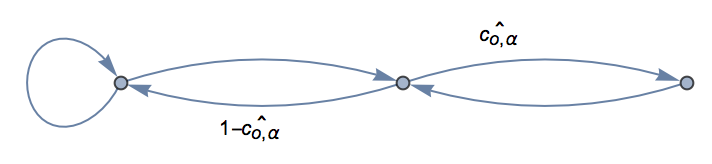
\includegraphics[width=0.5\textwidth]{p1.png}
\end{figure}

\textbf{Penalty Rule:} Assume this machine is working for floor $o$ (so $o$ is the floor last person gets off), it chooses to go to floor $\alpha$ to wait for next request, while the next person will get on floor $i$. Then the chance of getting penalty is:
$$\hat{c}_{o,i,\alpha}=\frac{T(o,i,\alpha)}{\sum_\alpha \hat{\mu}_{o,\alpha}}=\frac{T(o,i,\alpha)}{\sum_\alpha \sum_iT(o,i,\alpha)}$$

As discussed before, where
$$T(o,i,\alpha)=|i-\alpha|+\frac{1}{2}|o-\alpha|$$

To implement this, each time after we received the next person's choice $i$, we calculate $\hat{c}_{o,i,\alpha}$ and random a float number in $[0,1]$. Compare the random number with $\hat{c}_{o,i,\alpha}$, if the random number is smaller, we view this as a penalty, otherwise it is a reward.\\

So when we encounter $(o,i,\alpha)$, the probability of getting a penalty is $\hat{c}_{o,i,\alpha}P(I=i)$\\

Then the overall penalty probability of choosing $\alpha$ actually is (surprisingly!):

$$\frac{\sum_iT(o,i,\alpha)P(I=i)}{\sum_\alpha \hat{\mu}_{o,\alpha}}=\frac{\mu_{o,\alpha}}{\sum_\alpha \hat{\mu}_{o,\alpha}}=\hat{c}_{o,\alpha}$$

Recall that:
$$M_o=\frac{1}{\eta}\hat{M}_o=\frac{1}{\eta}\sum_\alpha \hat{c}_{o,\alpha} P(X_o=\alpha)$$

Based on Tsetlin theory, this scheme promises us an $\epsilon-optimal$ solution! (easy to show that when $k > 1$, $min(\hat{c}_{o,\alpha})<min(c_{o,\alpha}) \leq 0.5$)

Note that since each $\hat{c}_{o,i,\alpha}$ is relatively small, we need more states for Tsetlin machine for the sake of accuracy.
\subsubsection{FSSA and  Discretized}
Actually the above penalty rule can also be applied to $k-action$ FSSA and Discretized machine, the penalty probability still is $\hat{c}_{o,\alpha}$!

\subsubsection{Estimator}
While the Estimator algorithm is very different. An estimator of $P(I)$:

$$\hat{P}_I(n)=[\hat{p}_1(n),\hat{p}_2(n),...\hat{p}_k(n)]$$

Define $\hat{P}_I(0)=[\frac{1}{k},\frac{1}{k},...,\frac{1}{k}]$, each time after a get on/off event, we update $\hat{P}_I$. In this case we need to record history (which means we need a global memory to store this information).\\

Based on the fact that If we know $P(I)$, we know how to choose the best action:

For each $o \in O$, find:
$$\mu_{o,\alpha^*}=min(\mu_{o,\alpha})$$

Because $\mu_{o,\alpha} = \sum_iT(o,i,\alpha)P(I=i)$, this is only feasible when $P(I)$ is known.\\

We choose the best action $\alpha^*$ based on estimator $\hat{P}_I$, update the learning vector $P_{X_o}$:
$$P_{X_o}(n+1)=(1-a)P_{X_o}(n)+aP_{X^*}$$

Where $a\in [0,1]$ is a constant and $P_{x^*}[\alpha^*]=1$.\\

Since
$$\lim_{n\to \infty}\hat{P}_I(n)=P_I$$

Based on Estimator algorithm analysis, this can also give us an expedient solution!

\section{Simulation}
In the following simulation we use the following probability as basis:
\begin{verbatim}
var pi = []float64{0.1, 0.2, 0.3, 0.05, 0.2, 0.1, 0.05}
var po = []float64{0.15, 0.05, 0.15, 0.25, 0.05, 0.2, 0.15}
\end{verbatim}
pi is the probability vector of people get on floors, po is get-off probability vector and we use average $T$ as the performance measurement.

\subsection{Test Deduction}
We first test the correctness of deduction which is $E[T]_{min}=E[min(M_o)]=\sum_o\mu_{o,\alpha^*}P(O=o)$, find $\alpha^* \in \alpha$ that minimize the value of $\mu_{o,\alpha}$ (where $\mu_{o,\alpha} = \sum_iT(o,i,\alpha)P(I=i)$).\\

Repeat 10000 times:
\begin{figure}[H]
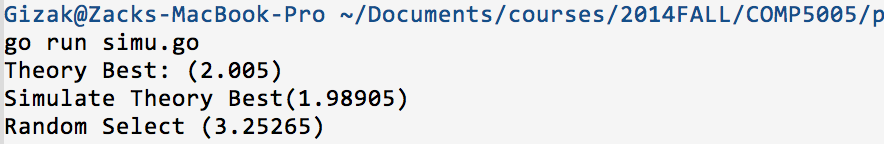
\includegraphics[width=0.6\textwidth]{p2.png}
\end{figure}

Repeat 100000 times:
\begin{figure}[H]
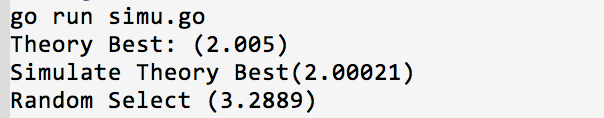
\includegraphics[width=0.5\textwidth]{p3.png}
\end{figure}

The ``Theory Best'' is computed using equation introduced before.\\

The ``Simulate Theory Best'' is using pi and po to compute the best actions at each floor, and then only use the selected action after one gets off.\\

The ``Random Select'' is actually ``do nothing'' scheme as a comparison, it just random selects the waiting floor.\\

We can see that the simulated data is very close to theory data, which gives us confident about the deduction part.

\subsection{Test Tsetlin}
Using the specific penalty rule to build Tsetlin machine. As we see, this scheme is not stable:
\begin{figure}[H]
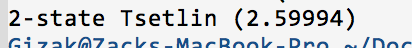
\includegraphics[width=0.4\textwidth]{p4.png}
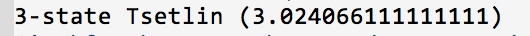
\includegraphics[width=0.5\textwidth]{p5.png}
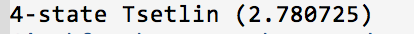
\includegraphics[width=0.4\textwidth]{p6.png}
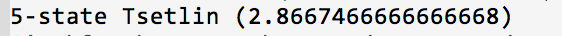
\includegraphics[width=0.5\textwidth]{p7.png}
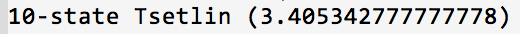
\includegraphics[width=0.5\textwidth]{p8.png}
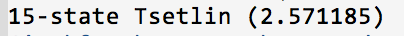
\includegraphics[width=0.4\textwidth]{p9.png}
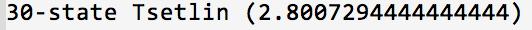
\includegraphics[width=0.5\textwidth]{p10.png}
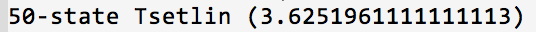
\includegraphics[width=0.5\textwidth]{p11.png}
\end{figure}

They use the common settings: repeat 1000000 times and calculate the average after 100000 iterations. One reason may cause this scheme unstable perhaps is that each penalty probability is very small and very close to each other, so make the environment noise-like and hard to learn. (does not preclude the programming errors...)
\subsection{Test Estimator}
The Estimator has the most accuracy:\\

Repeat 5000 times:
\begin{figure}[H]
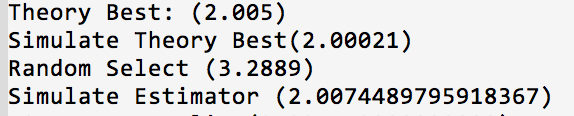
\includegraphics[width=0.6\textwidth]{p14.png}
\end{figure}

Repeat 10000 times:
\begin{figure}[H]
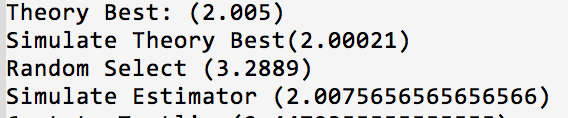
\includegraphics[width=0.6\textwidth]{p12.png}
\end{figure}

Repeat 20000 times:
\begin{figure}[H]
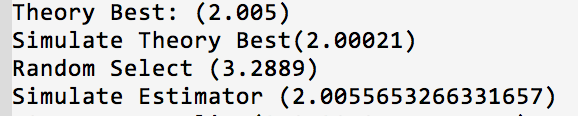
\includegraphics[width=0.6\textwidth]{p13.png}
\end{figure}

The simulated result is very close to theory best. This scheme uses estimated pi to compute the best action and move the action probability vector to approach the best action.

\emph{The code can be found at https://github.com/gizak/learning-automa}
\end{document}
